
%\renewcommand{\familydefault}{\sfdefault}
%=============== En−Tete ===============
 
%−−− Insertion de paquetages −−−−
\documentclass[12pt,a4paper]{report}
\usepackage[utf8]{inputenc}
\usepackage{amsmath}
\usepackage{amsfonts}
\usepackage{amssymb}
\usepackage{graphicx}
\usepackage{wrapfig}
\graphicspath{ {./images/} }
\usepackage[rightcaption]{sidecap}
\usepackage{subcaption}

\usepackage[french]{babel}
\usepackage[Bjarne]{fncychap}
\usepackage{fancyhdr}
\usepackage{float}
\usepackage{epsfig}
\usepackage{appendix}
\usepackage[final]{pdfpages}
\usepackage{array}
\usepackage{pdfpages}

\pagestyle{fancy}


\usepackage{titlesec}
%-\titleformat{\chapter}[display]{\bfseries}{\huge\chaptertitlename~\thechapter}{10pt}{\LARGE}--%

%−−− Page de garde - titre −−−

\begin{document}

\title{\Large{\Large {Travail de lecture et de rédaction scientifique sur le Federate Learning}}}

\author{Bal Sébastien}

\maketitle

\thispagestyle{empty} % Ignore page number

\fancyhead[LE,RO]{\leftmark}

\fancyhead[RE,LO]{}



 

%=============== Remerciement ===============

\begin{figure}[p]

\large\textbf{Remerciements}


\end{figure}

\tableofcontents
\thispagestyle{empty} % Ignore page number

\fancyfoot[C]{Master en Science infomatique - Lecture et rédaction scientifique}
\fancyfoot[R]{\thepage}

\chapter{Concepts}
\section{Machine Learning}
\thispagestyle{plain}\setcounter{page}{1} % Start page count
Le Machine Learning appelé en Français apprentissage automatique [x: wikipédiea] a pour objectif de traiter l'information afin de lui donner de la valeur ajoutée.\\

De nos jours, le Machine Learning est présent partout sur la toile, cela va du moteur de recherche comme Google, aux assistants vocaux comme Siri et Alexa, les fil d'actualités des réseaux sociaux comme Facebook et Twitter. Le point commun entre toutes ces platformes et le stockage massif des données de leur utilisateur appelé Big Data [x: ?]. Le Big Data est une technologie apparue dans les années xxxx, a permis l'essor de l'apprentissage automatique, le Machine Learning. En effet, cet imposant volume de données collectées sur les utilisateurs a permis, dans les exemples cités ci dessus, de mieux cibler le comportement des utilisateurs et donc améliorer les expériences.\\

Pour fonctionner, le Machine Learning(ML) a besoin de données à ingérer et d'avoir un modèle appris afin de fournir des données à valeur ajoutée comme des algorithmes de prédiction de bourse et la maintenance prédictive. Il est donc nécessaire d'identifier les solutions pour créer ces modèles de ML.\\

\begin{center}
	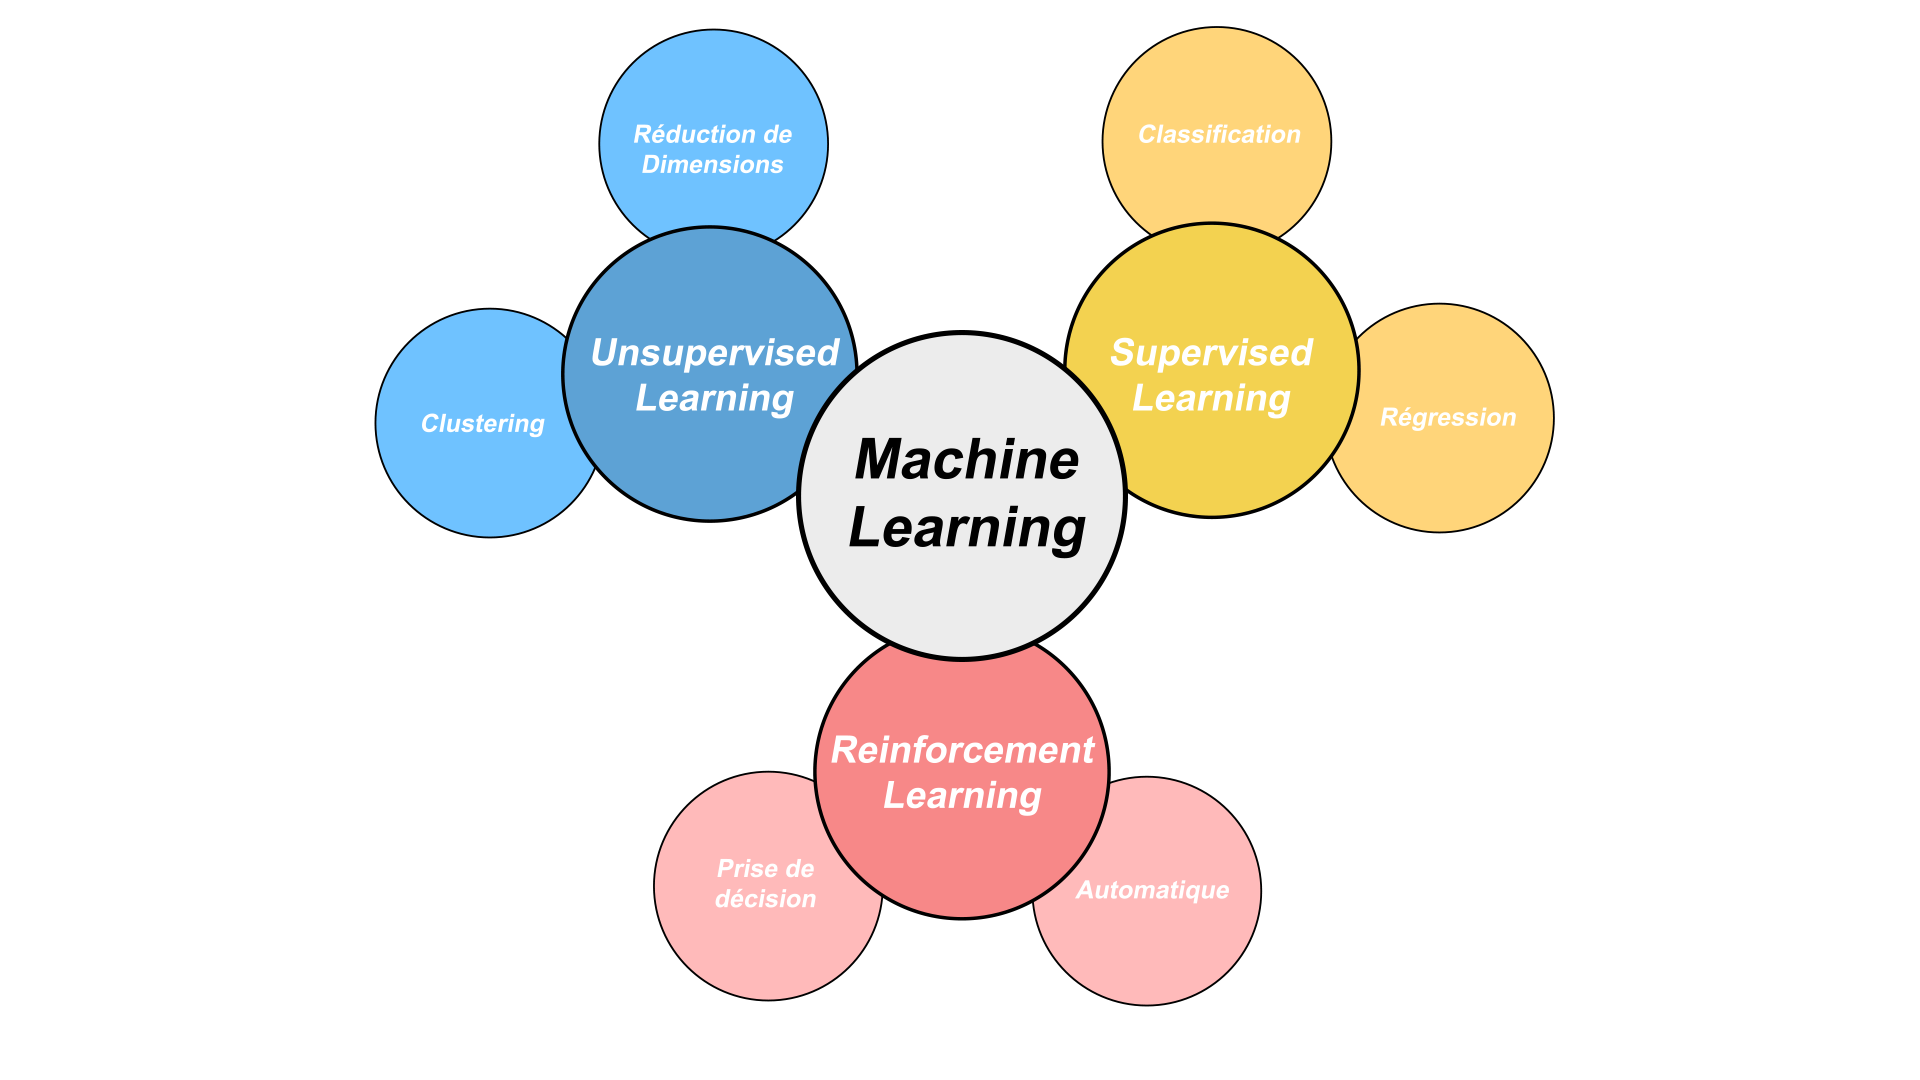
\includegraphics[scale=0.2]{ML_vignette}
	\captionof{figure}{Familles d'algorithmes les plus utilisés}
	\label{fig1}
\end{center}

La première famille, l'appentrissage supervisé (en jaune dans la figure 1.1) consiste à donner des données en entrées, le résultat attendu itéré sur un grand jeu de données afin de trouver la modèle. Pour que le modèle deviennent performant, on fournit un grand volume de données dans le but qu'il se rapproche du modèle attendu.\\

La deuxième famille,l'apprentissage non-surpervisé (en bleu dans la figure 1.1) consiste à apprendre par reconnaitre des ressemblances et des différences entre les données fournies. L'algorithme rassemble les données en groupe suivant ce qui lui semble le plus pertinant. Ainsi quand on passe un modèle bien précis à l'algorithme, il trouve plus facilement car il a été entrainé.\\

Pour finir, il existe une catégorie qui gère sa propre expérience. En effet, l'apprentissage par renforcement (en rouge dans la figure 1.1) consiste à générer ses propres expériences. On se rapproche de l'automobile autonome, la machine change ses états suivant les actions qu'elle entreprend de faire. Un système de récompense positive et négative est mis en place pour constituer une nouvelle expérience et rendre la machine attentive pour maximiser ses chances de réussite.\\
\pagebreak

Pour conclure, le ML est une technologie qui vise à trouver des modèles, comprendre des comportements afin de prédire les besoins d'une application suivant un utilisateur.\\

On peu constater que ce type de besoin se focalise sur une application spécifique cependant, le ML connait des limites au niveau des complexités combinatoire [x: ], or certaines applications nécessitent des applications plus complexes avec plus d'entrées, tels que le traitement des images. Pour palier aux limites du ML, le Deep Learning a vu son essort [x: lien vers essort DL]
\pagebreak



\section{Deep Learning}

Le Deep Learning(DL) est représentatif d'un système neuronal comme notre système cérébral, il est conçus de plusieurs neuronnes qui intéragissent entre eux. Pour rendre performant tous ces neuronnes, il est nécessaire d'avoir une grande quantité de données, un Data Lake. Celui ci fournit au système plusieurs informations afin de lui constituer une "mémoire". Cette mémoire lui permet de reconnaitre des éléments bien particulier suivant l'entrainement qu'il aura suivit. Cet entrainement est supervisé par des développeurs qui vérifient que le DL ne sort pas de son modèles définis.
Si il s'en éloigne, ils corrigent son algorithme mathématique pour le rendre performant et le remettre sur le droit chemin. Pour que le modèle mathématique deviennent performant, il faudra l'entrainer à reconnaitre une donnée en particulier. C'est le sujet de notre prochaine section.


\pagebreak

\subsection{Modèle d'entraînement}

Pour entrainer le DL, il lui faut un algorithme mathématique et un grand flux de données afin d'affiner ses recherches et prendre de l'expérience. Dans notre situation, on décider de prendre la reconnaissance d'une image, en particulier celle d'un chat.
On fournit à l'algorithme un flux d'images de plusieurs espèces d'animaux, on définit les paramètres qui permettent d'affirmer que l'image que l'on soumet soit bien un chat. Ainsi avec ces critères, l'algorithme devient plus précis car on le guide un peu sur l'objectif qu'il doit atteindre.
 
Voici un schéma pour l'exemple du fonctionnement du DL,[fig2.1], les boules vertes représente le bon chemin que le système va prendre pour arriver à vérifier le modèle qui était demandé. Les boules bleus sont celles qui ont des caractéristiques avec le modèle mais ne correspondra pas exactement au modèle qui était demandé. Les boules rouges quand à elles, représentent les erreurs que le système a exclu pour pouvoir apprendre le modèle exacte. Les erreurs sont par la suite renvoyées en amont du système pour que le système ajuste son modèle mathématique

\begin{center}
	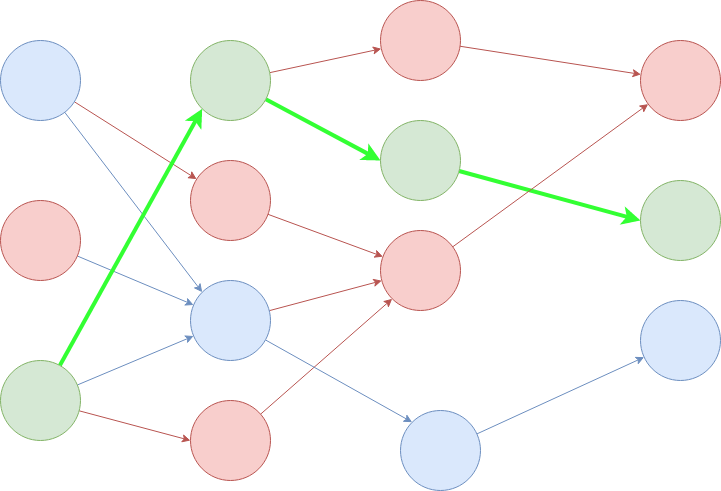
\includegraphics[scale=0.4]{deep_learning_schema}
	\captionof{figure}{Autoapprentissage Deep Learning}
	\label{fig1}
\end{center}

On peut constater que ce type d'algorithme peut être très vite devenir énergivore. De plus, le DL se focalise principalement sur une application. Or, il peut être intéressant d'étudier plusieurs applications similaires afin d'identifier des modèles plus poussés. C'est dans ce contexte que nous allons introduire le Federated Learning.


\section{Federated Learning}

Notre époque fait face à deux défis importants en terme d'avencer technologique: les respects des données des utilisateurs et l'augmentation du volume des données. L'une des plus importantes est celle de la privatisation de ces données sur le web. Avec la protection des données (RGPD) promulgué en 2018, les données privées font entièrement partie de l'utilisateur, ces données ne peuvent pas être utilisé sans son accord. Ensuite le silo des données met un frein à l'évolution de l'industrie moderne, c'est en ayant plus de données que l'on peut améliorer la qualité de la formation. Cependant le manque de données valides dans le domaine médical vient principalement du faite que les travailleurs doivent être expérimentés dans certains domaines comme celui de l'industrie médicale pour que la qualité des données soient au rendez vous.\\

C'est grâce au Federated Learning(FL) que l'essort de l'industrie a relevé ces défis. Car le FL est un processus d'apprentissage automatique qui vise a exploité les îlots de données tout en gardant la sécurité des données. Des clients sont coordonnées avec un ou plusieurs serveurs pour faciliter une décentralisation d'un appentrissage automatique. Le FL est lié aux deux concepts que nous avons vu précédements le Machine Learning et le Deep Learning, ce système distribué contient des calculs et des données tous les deux distribués. Le traitement distribué met en place plusieurs appareils connectés à différents endroits via un réseau de communication sous la surveillance d'un serveur centrale afin d'effectuer une partie de la même tâche pour l'accomplir. Le modèle distribué vise à améliorer l'étape de traitement comparer au FL qui lui se base sur un modèle collaboratif afin d'éviter des fuites de confidentialité.\\

Pour mieux comprendre son fonctionnement, le FL déroule en plusieurs étapes, la formation fédérée est celle qui est la plus courante. Pour commencer, un appareil mobile se procure un modèle en le téléchargeant afin d'avoir un formation suivie en local. En second lieu, le modèle téléchargé est subit à de multiple mises à jours régulière en local afin d'être amélioré, celles ci contiennent des données locales qui appartiennent à différents appareils séparés. Ensuite, ils téléchargent des informations d'un champ de vecteurs présent dans un cloud. En troisième lieu, les modèles locaux effectuent une mise à jour moyenne au sein du cloud et est envoyé à un appareil défini comme le modèle mondial renouvelé. Pour finir, ces étapes précédentes se répètent afin d'arriver à un modèle avec une certaine performance ou qu'une date limite soit atteinte.

Le FL est capable de traiter des données partionnées horizontalement suivant des echantillons et aussi de façon verticale suivant les caractéristiques du modèle d'apprentissage.

En quelques mots, c'est un apprentissage automatique distribué qui permet d'entraîner un modèle mathématique avec un large groupe de données décentralisées qui se trouvent sur des appareils distants. 

\pagebreak

\chapter{Technologies existantes (Framework)}
\subsection{TensorFlow Federated (TFF)}

Les frameworks ne manquent pas pour manipuler des modèles mathématique et les implémenter pour du ML. Le framework TensorFlow Federated en est un qui est totalement openSource. Il permet aux développeurs de simuler des algorithmes d'apprentissage sur leur modèles et bien entendu tester de nouveau algorithmes. Le TFF est constitué d'un environnement d'exécution de simulation dans lequel on peut simulé nos algorithmes, celle ci est utilisée par une seule machine dédiée aux tests.

\subsection{Federated AI Technology Enabler (FATE)}

\chapter{Catégorisation}

Le FL est caractérisé par trois grands groupes qui surviennet régulièrement, ceux ci sont le FL Horizontal, le FL vertical et le Federated Transfer Learning. Les données stockées sont placées dans différents noeuds, celles ci sont sous forme de matrice de caractéristiques. Les données sont composées de multiples instances, la partie horizontale est représentée comme un client, celle verticale se caractérise par les caractéristiques du client. Pour finir, on peut séparer le FL suivant le mode de partition des données.\\

\subsection{Horizontal FL}

Pour celui du FL Horizontal, des chevauchements peuvent apparaitrent entre les caractéristiques des données qui sont réparties sur différents noeuds, malgré le fait que les données ne sont pas semblables sur l'espace d'échantillonnage. Les données du point de vue de l'échantillonage sont différentes dans les scénarios des appareils connecté à Internet et les appareils intelligents. Mais ils sont particulièrment similaire dans un espace de fonctionnalité. Les mises à jours, comme nous l'avons vu précédement dans le point du FL, celle si est faite de façon horizontal. En effet, la dimension d'entité est la même pour chaque données. Dans les applications médicales, une forte hausse de travail est nécessaire pour collecté un grand nombre de données. Car il est difficile voir inconcevable pour chaque hôpital de créer une banque de données à partager. Via un réseau fédéral pour les hôpitaux construit par le FL permet d'améliorer le modèle(voir Fig 3.1).

\begin{center}
	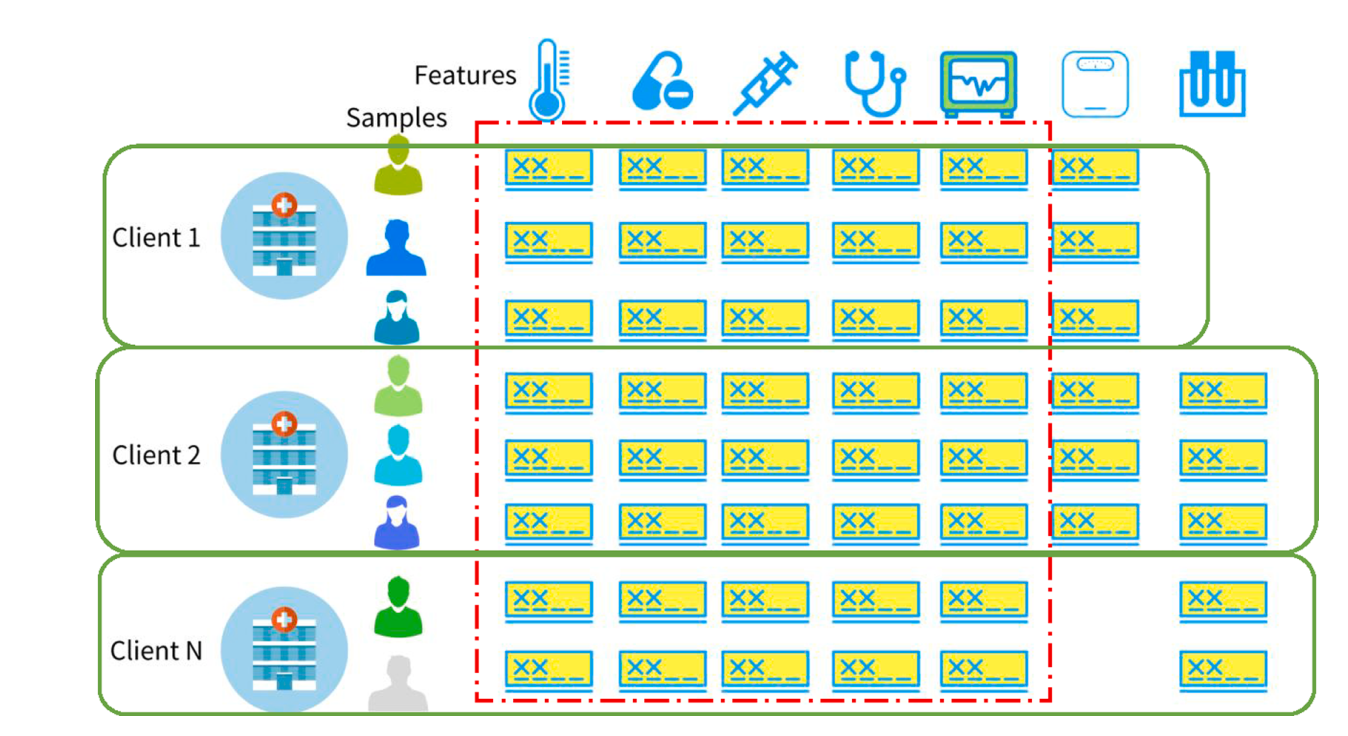
\includegraphics[scale=0.2]{fl_horizontal}
	\captionof{figure}{Horizontal FL}
	\label{fig1}
\end{center}


\subsection{Vertical FL}

Lorsque les données sont partitionnées, le FL vertical est plus approprié, chaque parties contient des données homogènes. Ce qui implique que les chevauchement se font en partie sur l'ID de l'échantillon alors qu'elle est différente dans l'espace fonctionnel. Prenons le cas d'un établissement médical, ils souhaitent identifier des maladies telles que le diabète. Il peut être analysé suivant certaines dimensions comme l'âge, le poids et les antécédants médicaux le type de diabète qu'un patient peut avoir. Avec le FL, certaines applications possèdent des données comme le nombre de pas ou la composition des plats qu'un personne a. Ces données peuvent être utilisées pour faciliter cette reconnaissance. La figure 3.2 illustre très bien le FL vertical.

\begin{center}
	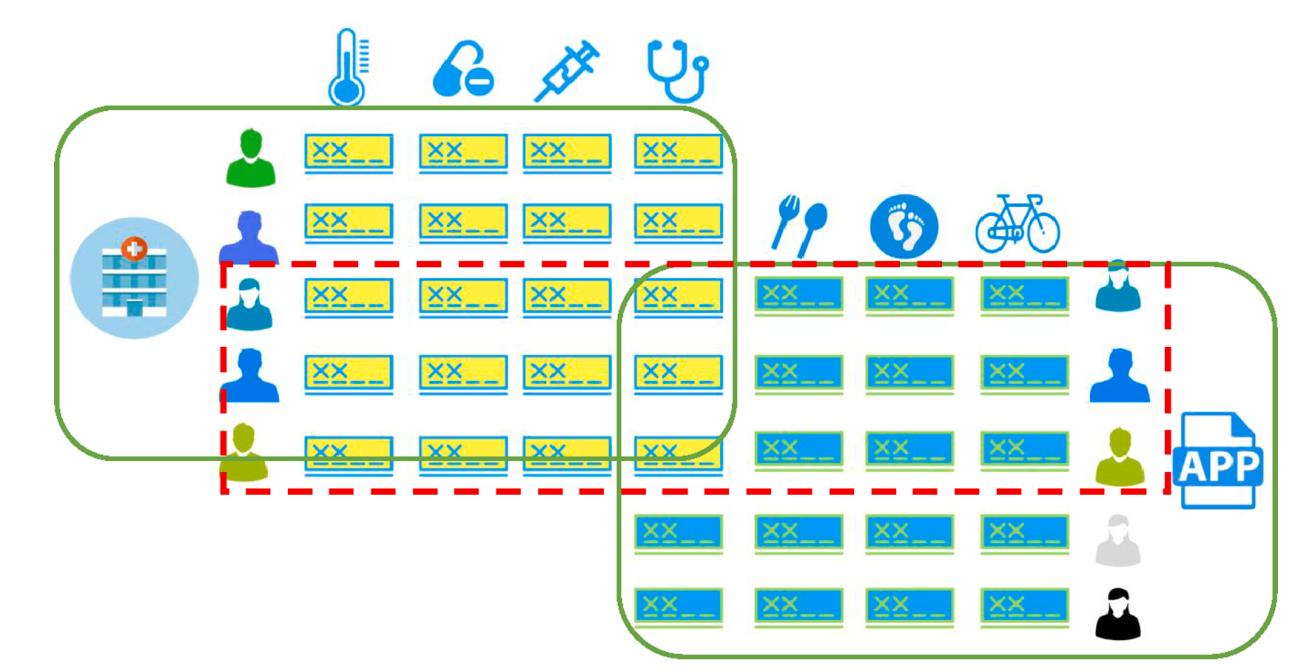
\includegraphics[scale=0.2]{fl_vertical}
	\captionof{figure}{Vertical FL}
	\label{fig1}
\end{center}
\pagebreak

\subsection{Federated Transfer Learning (FTL)}

En comparaison des deux scénarios vu précédement, dans la plupart des cituations, sur les espaces d'échantillonage et d'espace d'entité les données n'y sont pas partagées. Ce qui implique un manque d'étiquette et une mauvaise qualité des données. Le principe du FTL est transféré les données d'un domaine vers un autre afin de réaliser de meilleurs résultats d'apprentissage. Ainsi, le FTL permet d'avoir une application étendue pour ce qui est de parties communes avec des intersections étroites. Pour un système de réseaux de neuronnes qui possèdent une technologie de cryptage homomorphique peut empêcher des fuites de confidentialités mais aussi garder une très bonne précision. 

Dans le cadre d'une application avec le modèle FedHealth rassemble un packet de données qui appartiennent à des organisations différentes via FL et permet d'avoir un service personnalisé pour des soins de santé. Sur la Fig 3.3, des informations sur le diagnostic et le traitement de certaines maladies peuvent être partagées avec un autre hôpital dans le but de faciliter des diagnostics. Les problèmes qui surviennent à l'heure actuelle dans le milieu de l'industrialisation sont les îlots de données et la protection de la vie privée mais avec le FTL, celui ci permet d'avoir un service de sécurité fiable pour la protection des données et la confidentialité des utilisateurs tout en cassant les barreaux des îlots de données.

\begin{center}
	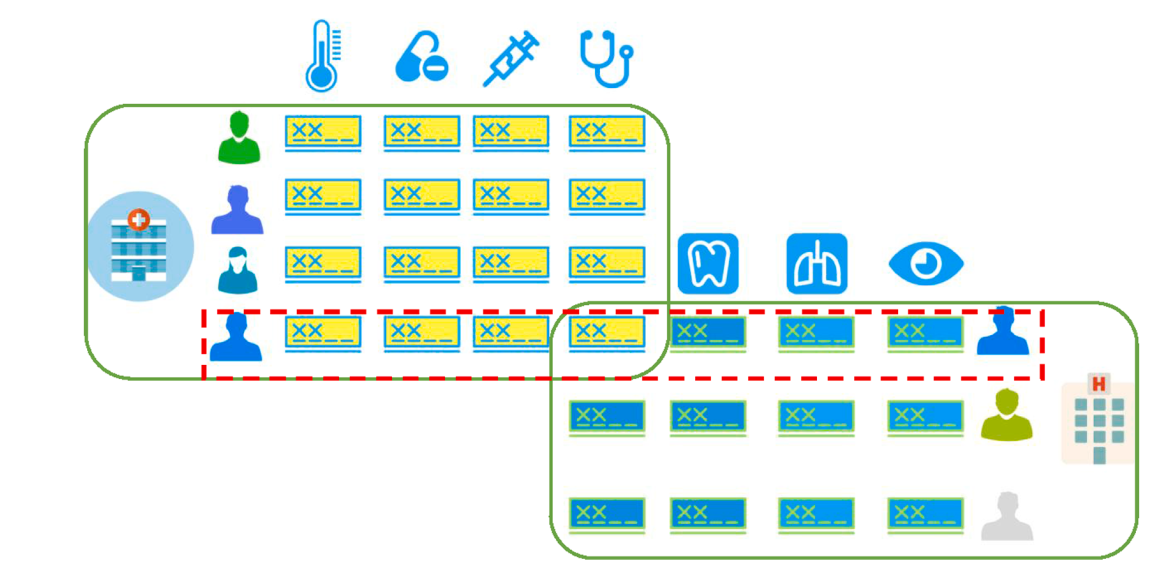
\includegraphics[scale=0.2]{fl_distribute}
	\captionof{figure}{FTL}
	\label{fig1}
\end{center}

\chapter{Exemples d'utilisations}

Dans notre société, le FL peut être un atout majeur pour plusieurs secteurs comme la finance, les soins de santé et l'éducation. Plusieurs applications qui peuvent faciliter les employers dans leur travail de tous les jours ou encore aider à la reconnaissance de certaines maladies et bien entendu aider nos têtes blondes pour améliorer et faciliter leur apprentissage pour qu'ils deviennent les hommes et les femmes de demain. Beaucoup de possibilités et pour se faire, un aperçu des ses applications dans lesquels il est possible d'utiliser le FL. 


Les deux problèmes qui surgissent sont la protection de la vie privée et la sécurité des données

\subsection{La Finance}

Le secteur de la finance est très important avec des réglementations gouvernementales pour la protection des investisseurs contre la fraude et la mauvaise gestion, conserver la confidentialité et la sécurités des données des utilisateurs. Dans le but de réduire les coûts et la charge de travail, des sociétés banquaires et financières exploitent les technologies modernes comme l'IA, les services de cloud et la technologie sur les téléphone mobile pour assurer un service financier de qualité tout en respectant les réglementations gouvernemantales. Un cas bien particulier est le financement intelligent à la consomation, son objectif vise à prendre parti des techniques de ML afin de proposer des services financiers propre à chacun. Les données utilisées dans un crédit à la consommation sont fait d'informations sur les consommateurs comme le pouvoir d'achat, le préférence d'achat et aussi les caractéristiques du produit. Ces données peuvent être utilisée par diversses entreprises ou sociétés. Ainsi dans la Figure xxx, les informations de qualifications et le pouvoir d'achat peuvent être déduit de son épargne bancaire et de sa préférence d'achat sur des produits ou services. On fait face dans notre exemple à deux problèmes. Le premier est la protection de la vie privé des consommateurs et le sécurité des données barrière entre les banques, les réseaux sociaux, les sites d'e-commerce. Le deuxième, ce sont le stockages des données par trois sections sont hétérogènes, ce qui empêche le ML classique de fonctionner sur des données hétérogènes. C'est pour cette raison que le FL résout ces problèmes. Le FL peut scinder les données en trois parties sans exposer les données. On peut aussi utiliser l'apprentissage par transfert pour examiner les données hétérogène.

\begin{thebibliography}{9}

	\bibitem{lamport94}
	  Leslie Lamport,
	  \emph{\LaTeX: A Document Preparation System}.
	  Addison Wesley, Massachusetts,
	  2nd Edition,
	  1994.
	  
	\bibitem{LiliYuxiTseLin}
	  Li Li, Fan de Yuxi, Mike Tse, Kuo-Yi Lin,
	  \emph{\LaTeX: A review of applications in federated leaning}.
	  Comuters and Industrial Engineering,
	  Volume 149,
	  November 2020,
	  106854
	  
	  \bibitem{FL_synthesis}
	  Qiang Yang, Yang Liu, Yong Cheng, Yan Kang, Tianjian Chen, Han Yu
	  \emph{\LaTeX: Federated Learning, Synthesis Lectures on Artificial Intelligence and Machine Learning}.
	  Ronald J. Brachlan, Francesca Rossi and Peter Stone,
	  Morgan and Claypool publishers,
	  Series Editors
	  December 2019
	  
	\bibitem{bigdata}
	Pour la partie sur le Machine Learning https://www.lebigdata.fr/machine-learning-et-big-data

\end{thebibliography}


\label{Pour la partie sur le Machine Learning https://www.lebigdata.fr/machine-learning-et-big-data}

\label{TensorFlow : https://www.lebigdata.fr/tensorflow-definition-tout-savoir}

%Citeseer citeseer.ist.psu.edu,Google Scholar scholar.google.com,ScienceDirect www.sciencedirect.com,ACM Digital Library portal.acm.org,IEEE Digital Library www.computer.org/portal/site/csdl/index.jsp
 


\begin{appendix}
 \chapter{Annexe}
 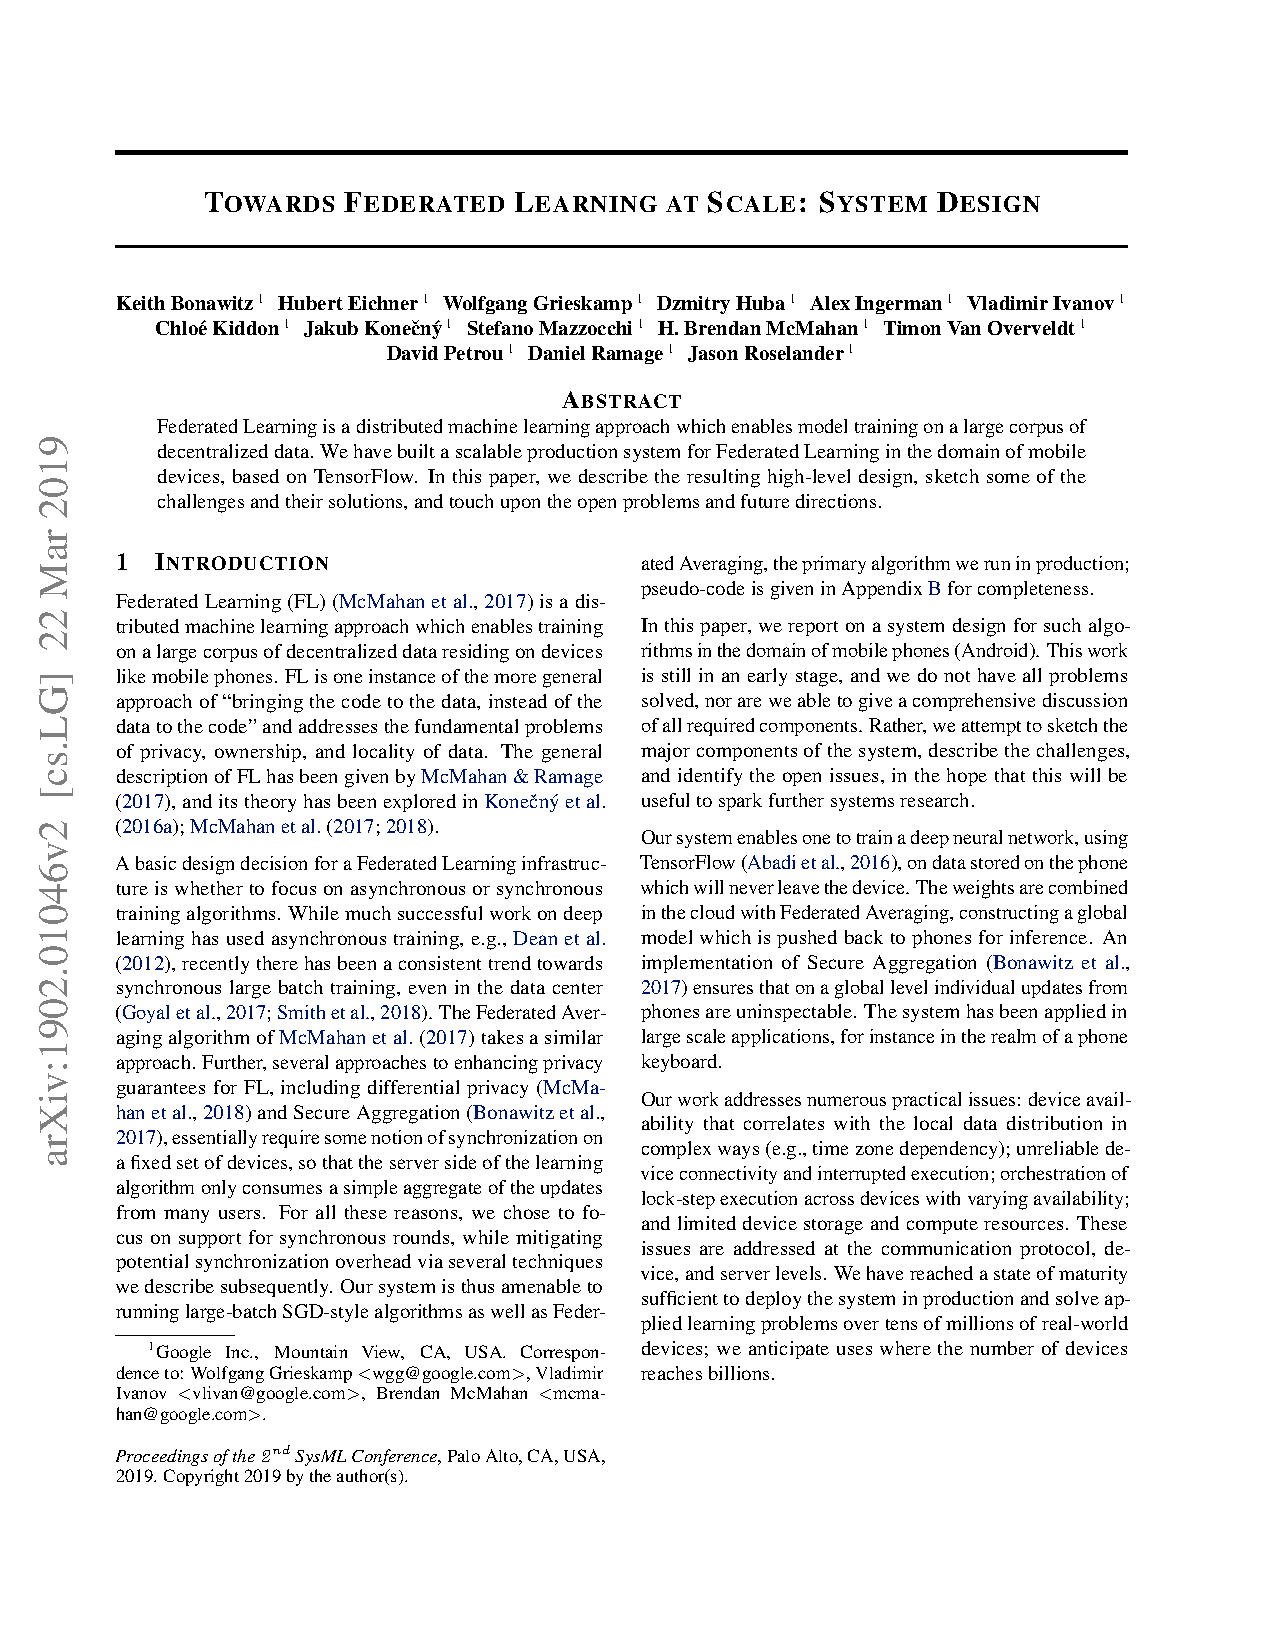
\includepdf{pdf/federate_learning_en.pdf}
\end{appendix}

\end{document}
